\documentclass[conference,a4paper]{IEEEtran}
% IEEE conference layout, retaining the assignment's A4 paper size.
\widowpenalty=10000
\clubpenalty=10000
\usepackage[utf8]{inputenc}
\usepackage[T1]{fontenc}
\usepackage{cite}
\usepackage{amsmath,amssymb,amsfonts}
\usepackage{algorithmic}
\usepackage{graphicx}
\usepackage{textcomp}
\usepackage{xcolor}
\usepackage{booktabs}
\usepackage{tabularx}
\usepackage{makecell}
\usepackage{listings}
\usepackage{tikz}
\usepackage{float}
\usetikzlibrary{positioning,arrows.meta}
\usepackage[hidelinks]{hyperref}
\usepackage{url}
\usepackage{comment}
% IEEEtran supplies the title, heading, caption and column spacing.
% For future subfigures, use subfig with caption=false rather than subcaption.
\def\BibTeX{{\rm B\kern-.05em{\sc i\kern-.025em b}\kern-.08em
    T\kern-.1667em\lower.7ex\hbox{E}\kern-.125emX}}

% Reduce vertical whitespace around displayed equations
\setlength{\abovedisplayskip}{4pt}
\setlength{\belowdisplayskip}{4pt}
\setlength{\abovedisplayshortskip}{2pt}
\setlength{\belowdisplayshortskip}{2pt}
\raggedbottom
\interdisplaylinepenalty=2500

\begin{document}

\title{ELEC3304 Assignment: A Self-Balancing Controller for Microducks}

\author{\IEEEauthorblockN{Alec Doherty}
\IEEEauthorblockA{\textit{Faculty of Engineering}\\
\textit{The University of Sydney}\\
Sydney, Australia\\
Student ID: 541029627}
\and
\IEEEauthorblockN{Parvez Manahan}
\IEEEauthorblockA{\textit{Faculty of Engineering}\\
\textit{The University of Sydney}\\
Sydney, Australia\\
Student ID: 540897492}
}

\maketitle

\begin{abstract}
Small bipedal robots are inherently unstable when standing and require continuous feedback to maintain balance. This paper investigates standing balance and push recovery for the MicroDuck using a nonlinear multibody simulation model. The robot is modelled as a floating-base system with eight actuated leg joints, first-order servo dynamics and compliant foot--ground contact. Linearisation about a crouched standing equilibrium produces a 33-state balance model with one unstable pole at $+2.90$~rad/s. Two controllers are developed and compared: coordinated roll--pitch PID control and observer-based state feedback using pole placement. Both generate joint-angle targets for the position-controlled servos at 50~Hz. A discrete observer estimates unmeasured body and joint velocities and servo torques from gyroscope, accelerometer and encoder measurements. Performance is evaluated using the full nonlinear model, including actuator lag, saturation, ground contact, external disturbances and sensor imperfections. The study compares recovery, disturbance rejection and estimation performance, highlighting the challenges of applying linear control methods to nonlinear, contact-constrained bipedal systems.
\end{abstract}

\begin{IEEEkeywords}
MicroDuck, standing balance, inverted pendulum, state feedback, state observer, integral control
\end{IEEEkeywords}

\section{Introduction}
Maintaining balance is a fundamental requirement for bipedal robots, as instability can prevent standing and walking behaviours. This report investigates standing balance control for the MicroDuck, a biped about 25~cm tall with 15 servos~\cite{openmicroduck_params} and a simulation-model mass of about 0.74~kg~\cite{pollen_mjcf}. The robot's small scale and servo-based actuation present challenges for stabilisation, particularly when gravitational effects produce destabilising dynamics. Regulating body roll and pitch provides a first step for stable standing.

Several modelling approaches exist for balancing systems. The linear inverted pendulum model treats a bipedal robot as a point mass on a massless leg with constant height, which gives linear dynamics that suit analysis and design~\cite{kajita2001}. However, this simplification neglects angular momentum~\cite{stephens2007}. More detailed balance strategies combine ankle control, hip motion and stepping to improve balance recovery capability~\cite{stephens2007,aftab2012}. These reduced order approaches can also be related to the full multibody dynamics, where joint torques act on a floating base motion through ground contact~\cite{tedrake_multibody}.

Existing control approaches involve trade-offs between implementation complexity and performance. Linear feedback on an inverted pendulum with saturated ankle torque is simple to implement and analyse~\cite{stephens2007}, but it is valid only near the operating point and does not handle constraints directly. Model predictive control can incorporate support constraints and combine ankle, hip and stepping strategies within a unified optimisation framework~\cite{aftab2012}, but it needs online optimisation. Deep reinforcement learning has produced agile behaviour on a miniature humanoid with zero-shot transfer~\cite{haarnoja2024}, but relies on randomisation and perturbations in training rather than analytical guarantees. Since MicroDuck itself uses a learned policy~\cite{openmicroduck_params}, a model-based controller provides a useful alternative for investigating the robot's balance dynamics.

This report develops an observer-based state-feedback controller for MicroDuck standing balance using a floating-base rigid-body model incorporating actuated leg joints, servo dynamics and compliant foot contact. The nonlinear model is linearised about the standing equilibrium to obtain an LTI state-space representation for controller and observer design. Controller performance is subsequently evaluated through numerical simulations of the nonlinear system under realistic operating conditions. The remainder of this report presents the system model, problem definition, controller design and numerical validation, followed by conclusions.



\section{System Model}
\subsection{Platform and Modelling Scope}
MicroDuck's kinematic and inertial model is published by the manufacturer~\cite{pollen_mjcf}, while its runtime architecture and 50~Hz control loop are documented independently~\cite{openmicroduck,openmicroduck_params}. This study considers standing balance and push recovery using a simplified rigid-body simulation, rather than a calibrated model of production hardware. Link masses are taken from the published model \cite{pollen_mjcf}, but link geometry, centre of mass (COM) positions, and contact parameters are simplified assumptions (Table~\ref{tab:params}). 

The model has nine bodies: a merged upper body (torso, neck, head) and four per leg (hip-roll carrier, thigh, shin, foot). Hip yaw, neck and head joints are fixed, leaving eight actuated leg joints. The torso is a floating base with six degrees of freedom, giving 14 generalised coordinates $\mathbf{q}=[X,Y,Z,\psi,\theta,\phi,\mathbf{q}_j^\top]^\top$, where $X,Y,Z$ denote the torso position, $\psi,\theta,\phi$ are yaw, pitch and roll (Euler angles, $R=R_z(\psi)R_y(\theta)R_x(\phi)$), and $\mathbf{q}_j\in\mathbb{R}^8$ are the joint angles, ordered left then right (hip roll, hip pitch, knee and ankle). The generalised velocity $\dot{\mathbf{q}}$ contains the Euler-angle rates, which are distinct from the physical angular velocity of the torso. World axes are $X$ forward, $Y$ left and $Z$ up. Walking is not modelled. Instead, disturbances representative
of gait-related body moments are introduced as external wrenches.


\subsection{Nonlinear Dynamics}
The 36-dimensional state and eight-dimensional input are
\[
\mathbf{x}=[\mathbf{q}^\top,\dot{\mathbf{q}}^\top,
\boldsymbol{\tau}^\top]^\top,\qquad
\mathbf{u}\in\mathbb{R}^8,
\]
where $\boldsymbol{\tau}$ denotes delivered servo torque and $\mathbf{u}$ denotes commanded joint angles. The rigid-body equations for the nine-body system follow the Euler--Lagrange formulation~\cite{tedrake_multibody}, with first-order servo torque dynamics:
\begin{equation*}
\label{eq:servo}
\begin{gathered}
M(\mathbf{q})\ddot{\mathbf{q}}
+ \mathbf{h}(\mathbf{q},\dot{\mathbf{q}})
+ D\dot{\mathbf{q}}
= S\boldsymbol{\tau} + Q_c(\mathbf{q},\dot{\mathbf{q}})
+ \Gamma(\mathbf{q})\,\mathbf{w}, \\
\mathbf{u}_{\mathrm{lim}}
=
\operatorname{clip}
(\mathbf{u},\mathbf{u}_{\min},\mathbf{u}_{\max}),\\
T_a\dot{\boldsymbol{\tau}}
=
\operatorname{clip}\big(
K_p(\mathbf{u}_{\mathrm{lim}}-\mathbf{q}_j)
-K_d\dot{\mathbf{q}}_j,
-\boldsymbol{\tau}_{\max},
\boldsymbol{\tau}_{\max}
\big)
-\boldsymbol{\tau}.
\end{gathered}
\end{equation*}
Here $M$ is the mass matrix, $\mathbf{h}$ contains Coriolis, centrifugal and gravitational terms, $D=\operatorname{blkdiag}(0_{6\times6},\operatorname{diag}(b_j))$ represents joint damping, and $S=[0_{8\times6}\;I_8]^\top$ selects the actuated coordinates (the six floating coordinates have no direct actuator). $Q_c$ is the generalised contact force, and $\mathbf{w}=[F_x,F_y,F_z,N_x,N_y,N_z]^\top$ is an external world-frame wrench applied at the torso origin. $K_p$, $K_d$ and $T_a$ are diagonal $8 \times8$ matrices containing servo gains and torque time-constants, while $\tau_{\text{max}}$ defines the joint torque limits. Both command-angle and torque saturation are applied element-wise. The internal servo loop is part of the plant; the outer controller therefore adjusts $\mathbf{u}$ about its equilibrium value.

Ground contact is modelled at four sole corners per foot. For a contact point below the ground plane ($z<0$), the normal and tangential forces are
\begin{equation*}
f_n=\max(0,-k_nz-c_n\dot z),\qquad \mathbf{f}_t=-\mu f_n\frac{\mathbf{v}_t}{\sqrt{\|\mathbf{v}_t\|^2+v_s^2}},
\end{equation*}
with $f_n=0$ for $z\geq0$. The forces are mapped into $Q_c$. Since contact can only push, the corner forces bound the ground-reaction moment and hence tipping resistance. %Because the ground can only push upwards on the feet, not pull them down, the forces at the four corners of each foot determine how much turning force the foot can generate. The four corner contacts also constrain the available ground-reaction moments and hence the robot's resistance to tipping. 
Friction regularisation uses $v_s=5$~mm/s, permitting small tangential creep, and contact switching makes the dynamics piecewise smooth.

The model neglects collisions, mechanical joint stops, motor electrical and thermal dynamics, and additional joint compliance. Link inertias use uniform-box approximations. The official simulation includes approximately $\pm1^\circ$ gear backlash and a 3--6-step actuator delay (60--120~ms at 50~Hz) ~\cite{openmicroduck_sim}. These effects and the 50~Hz sample-and-hold are considered in numerical validation rather than the continuous-time plant. Euler-angle coordinates limit validity to moderate tilts, so simulations terminate at $20^\circ$ tilt or when hip height falls below 0.06~m.



\subsection{Standing Equilibrium and Parameters} 
The selected symmetric standing posture uses hip pitch, knee and ankle angles of $-20^\circ$, $40^\circ$ and $-20^\circ$, respectively, with zero hip roll. Newton iteration determines an equilibrium torso height of 0.122~m and near-zero pitch and roll, with all eight sole corners loaded. Static joint torques determine the servo targets, $\mathbf{u}_{eq}=\mathbf{q}_{j,eq}+\boldsymbol\tau_{eq}\oslash \mathrm{diag}(K_p)$. The largest static torque is 0.049~N\,m at the knees (approximately 8\% of the torque limit), and the minimum corner load is 0.85~N. At $K_p=0.55$~N\,m/rad, this torque requires a $5.1^\circ$ position error. The resulting knee and ankle targets are therefore $34.9^\circ$ and $-19.4^\circ$, respectively. The whole-body COM is 0.139~m above ground and 1.6~mm ahead of the ankle axis. The sole corners span $-27.1$ to $+26.9$~mm in $X$ and $\pm60.5$~mm in $Y$ about the torso origin, corresponding to approximate rigid-body tipping angles of $10.3^\circ$ forward, $11.7^\circ$ backward and $23.6^\circ$ sideways. The sideways value exceeds the $20^\circ$ model-validity limit.

This equilibrium is a modelling choice, not the runtime home pose, which specifies joint-specific angles and sign conventions for matching training reference frames~\cite{openmicroduck_params}. 
%This equilibrium is a modelling choice rather than the manufacturer's runtime home pose, whose joint angles use different reference frames and axis conventions~\cite{openmicroduck_params}. 

\begin{table}[H]
\centering
\caption{Model parameters (nominal value and sweep range).}
\label{tab:params}
\setlength{\tabcolsep}{3pt}
\renewcommand{\arraystretch}{1.05}
\resizebox{\columnwidth}{!}{%
\begin{tabular}{llll}
\hline
Symbol & Value & Range & Source \\
\hline
$m$ (total) & 0.737 kg & $\pm5\%$ & MJCF link masses~\cite{pollen_mjcf} \\
Upper-body mass & 0.479 kg & $\pm5\%$ & MJCF, trunk+neck+head~\cite{pollen_mjcf} \\
Upper-body COM height & 55 mm & $\pm8$ mm & assumed; informed by trunk CoM randomisation~\cite{openmicroduck_sim}\\
Whole-body COM height & 0.139 m & -- & derived at trim \\
Thigh, shin length & 50, 50 mm & -- & assumed (simplified) \\
Foot size & $54\times41$ mm & -- & assumed (simplified) \\
$K_p$ & 0.55 N\,m/rad & 0.386--0.55 & calibrated sets~\cite{microduck_rl_joints,microduck_actuator_selection} \\
$K_d$ & 0 N\,m\,s/rad & 0--0.053 & firmware D=0~\cite{openmicroduck_params}; checked separately \\
$b_j$ & 0.053 N\,m\,s/rad & 0.041--0.053 & calibrated sets~\cite{microduck_rl_joints,microduck_actuator_selection} \\
%$T_a$ & 0.03 s & 0.02--0.08 & runtime filter, 17--56 ms~\cite{openmicroduck_sim} \\
$T_a$ & 0.03 s & 0.02--0.08 & assumed actuator lag; sensitivity sweep \\
$\tau_{\max}$ & 0.60 N\,m & -- &
Inferred from XL330-M288-T stall torque at 6 V~\cite{robotis_xl330} \\
$k_n,c_n$ (per corner) & 4000 N/m, 12 N\,s/m & -- & assumed (0.23 mm static sag) \\
$\mu$ & 0.6 & -- & assumed; official sim: 1.0~\cite{openmicroduck_sim} \\
$v_s$ & 5 mm/s & -- & numerical regularisation \\
\hline
\end{tabular}}
\end{table}

%The total and upper-body masses (0.737 and 0.479~kg) are taken from the published MJCF model~\cite{pollen_mjcf}. Link geometry, COM location and contact properties are simplified assumptions. The nominal friction coefficient is $\mu=0.6$, compared with 1.0 in the official simulation ~\cite{openmicroduck_sim}.

The $\pm0.60$~N\,m torque limit is based on the XL330-M288-T stall-torque specification at 6~V ~\cite{robotis_xl330}. This is a peak rating, and the installed actuator variant has not been independently confirmed. Servo stiffness and joint damping are based on actuator configurations published in the official MicroDuck RL repository~\cite{microduck_rl_joints}. Nominal $K_d=0$ reflects the firmware derivative setting ~\cite{openmicroduck_params}. The 81-case sweep covers $m$, COM height, the $K_p$--$b_j$ pair and $T_a$ (Table~\ref{tab:params}). $K_d$ is varied one at a time at nominal.
%The 81-case sweep covers the $m$, COM-height, $K_p$ and $T_a$ ranges in Table~\ref{tab:params}.


\subsection{Actuation, Disturbances and Sensors}
All eight leg servos are available for balance control. The plant imposes a $\pm0.60$~N\,m torque limit and joint command ranges of $\pm20^\circ$ (hip roll), $-57^\circ$ to $34^\circ$ (hip pitch), $3^\circ$ to $86^\circ$ (knee), $\pm46^\circ$ (ankle), narrower than the given $\pm22^\circ$, $\pm90^\circ$ in~\cite{openmicroduck_params}.
%The plant enforces a $\pm0.60$~N\,m torque limit and joint command ranges of $\pm20^\circ$ (hip roll), $-57^\circ$ to $34^\circ$ (hip pitch), $3^\circ$ to $86^\circ$ (knee) and $\pm46^\circ$ (ankle), narrower than the official model limits~\cite{openmicroduck_params}. 
Disturbances are applied as configurable world-frame wrenches $\mathbf{w}$ at the torso origin, including Gaussian and rectangular pushes, steps and sinusoidal loads. Since the torso origin is approximately 0.12~m above ground, horizontal forces also generate moments about the feet. The linear inverted pendulum ankle-balancing model gives a maximum recoverable velocity without stepping of $v_{\max}=x_m\sqrt{g/h}\approx 0.21$~m/s, using $h=0.139$~m and a forward support margin $x_m=25$~mm~\cite{stephens2007}. Thus, a $0.05$~m/s disturbance is geometrically modest, although actual recovery also depends on servo torque, actuator dynamics, contact and friction. The official walking pushes of up to $\pm0.3$~m/s every 3--6~s~\cite{openmicroduck_sim} exceed this and would need stepping.

The measurement vector is $\mathbf{y}=[\boldsymbol\omega_b^\top, \mathbf{a}_b^\top,\mathbf{q}_j^\top]^\top \in\mathbb{R}^{14}$. 
It comprises three-axis gyroscope and accelerometer readings and eight joint encoder angles, giving 14 measurements. The LSM6DSV16X IMU is sampled at 50~Hz~\cite{openmicroduck_params,lsm6dsv16x}. Unlike the deployed sensor-fusion implementation, this model uses raw accelerometer specific force to avoid introducing unpublished filter dynamics and latency.

Measurement errors are modelled as
\[
\mathbf{y}_m=
\mathrm{blkdiag}(R_m,R_m,I_8)\mathbf{y}
+\mathbf{b}+\mathbf{n},
\]
where $R_m$ represents fixed IMU mounting misalignment (up to $6^\circ$), $\mathbf{b}$ contains constant sensor biases, including encoder offsets up to 0.015~rad, and $\mathbf{n}$ represents white measurement noise. IMU noise densities from the manufacturer's datasheet~\cite{lsm6dsv16x}, integrated over an assumed 25~Hz bandwidth, give nominal RMS levels of $0.014^\circ$/s for the gyroscope and 2.9~mm/s$^2$ for the accelerometer. Stress tests additionally use $2^\circ$/s and 0.1~m/s$^2$ noise, respectively. Additional error settings are given in Appendix~\ref{app:sensors}.

Only 14 measurements are available for the 36-state system. Joint velocities, body velocities and delivered servo torques are unmeasured and must be reconstructed by the observer. Absolute position and yaw are not directly observable and are not required for balance regulation.


\section{Problem Definition}

\subsection{Control Aims}
The model is open-loop unstable, with one real pole at $+2.90$~rad/s. This pole remains positive across all 81 parameter combinations, ranging from $+1.99$ to $+5.06$~rad/s. At nominal, raising $K_d$ to 0.053 slows it to $+1.94$~rad/s, so $K_d=0$ is the worst case. A $2^\circ$ initial tilt reaches $5^\circ$ in approximately 0.32~s, requiring rapid feedback stabilisation.

The controller must regulate roll and pitch, recover from disturbances, track lean references and reject constant external moments while respecting actuator and contact constraints. Since only IMU and encoder measurements are available, unmeasured states require observer estimation. Integral action is introduced to remove steady-state tracking and constant-disturbance errors.


\subsection{Operating Point and Linear Model}

The model is linearised about the symmetric crouched standing equilibrium $\mathbf{x}_{eq},\mathbf{u}_{eq}$ established in the System Model section, with $\mathbf{w}=0$. The selected posture uses approximately $40^\circ$ knee flexion, maintaining all eight foot contact points while keeping joint commands and static torques within their limits. This provides a representative standing configuration without placing the knees near their minimum command limit.

Hereafter, $\mathbf{x}$, $\mathbf{u}$ and $\mathbf{y}$ denote deviations from equilibrium. The linearised model is
\[
\dot{\mathbf{x}}=A\mathbf{x}+B\mathbf{u}+B_d\mathbf{w},
\qquad
\mathbf{y}=C\mathbf{x}+D_w\mathbf{w},
\]
where $\mathbf{x}\in\mathbb{R}^{36}$, $\mathbf{u}\in\mathbb{R}^{8}$, $\mathbf{w}\in\mathbb{R}^{6}$ and $\mathbf{y}\in\mathbb{R}^{14}$. The matrices are obtained using central finite differences of the nonlinear plant and IMU measurement model. The encoder rows of $C$ are constructed analytically, while the IMU rows are obtained by linearising the gyroscope and accelerometer measurements. The disturbance enters the mechanical accelerations through
\[
B_d=\begin{bmatrix}0\\M_0^{-1}\Gamma_0\\0\end{bmatrix},
\qquad \Gamma_0=\Gamma(\mathbf{q}_{eq}),
\]
and $D_w$ accounts for the direct effect of the wrench on accelerometer measurements. The observer does not explicitly model the disturbance.

The mechanical structure of the linearised system is
\begin{equation*}
\begin{aligned}
A&=
\begin{bmatrix}
0&I_{14}&0\\
-M_0^{-1}\mathcal{K}_{\mathrm{eff}}
&-M_0^{-1}\mathcal{D}_{\mathrm{eff}}
&M_0^{-1}S\\
-T_a^{-1}K_pS^\top
&-T_a^{-1}K_dS^\top
&-T_a^{-1}
\end{bmatrix},\\
B&=\begin{bmatrix}0\\0\\T_a^{-1}K_p\end{bmatrix},
\qquad
C=\begin{bmatrix}
C_{\mathrm{imu}}\\
0_{8\times6}\quad I_8\quad 0_{8\times22}
\end{bmatrix}.
\end{aligned}
\end{equation*}
Here $M_0=M(\mathbf{q}_{eq})$, $\mathcal{K}_{\mathrm{eff}}=\partial(\mathbf{h}_g-Q_c)/\partial\mathbf{q}$ and $\mathcal{D}_{\mathrm{eff}}=D-\partial Q_c/\partial\dot{\mathbf{q}}$, evaluated at equilibrium. $C_{\mathrm{imu}}$ is the linearised six-axis IMU measurement model, including the dependence of accelerometer measurements on system acceleration. The encoder rows directly measure the eight joint angles. There is no direct control feedthrough. This local model assumes inactive actuator saturation and fixed contact; saturation and contact switching are retained in nonlinear validation.

Absolute position $X,Y$ and yaw $\psi$ do not affect the balance dynamics and are not required as regulated outputs. Removing these three coordinates, while retaining their velocities, gives a 33-state balance subsystem. Let $T\in\mathbb{R}^{33\times36}$ select the remaining states:
\[
\begin{aligned}
\mathbf{x}_b&=T\mathbf{x},&
A_b&=TAT^\top,& B_b&=TB,\\
B_{d,b}&=TB_d,& C_b&=CT^\top,& D_{w,b}&=D_w.
\end{aligned}
\]
Thus,
\[
\mathbf{x}_b=
[Z,\theta,\phi,\mathbf{q}_j^\top,
\dot{\mathbf{q}}^\top,\boldsymbol{\tau}^\top]^\top
\in\mathbb{R}^{33}.
\]
The regulated output is torso roll and pitch,
\[
\mathbf{z}=[\phi,\theta]^\top=C_z\mathbf{x}_b,
\qquad C_z=[e_3^\top;\,e_2^\top].
\]
The removed position and yaw states are unobservable from the selected measurements. Small numerical residuals in the yaw-related columns (at most $1.8 \times 10^{-7}$) are treated as numerical error.
%(maximum approximately $1.76\times10^{-7}$ in $A$ and $8.88\times10^{-10}$ in $C$) are treated as numerical errors.

The nominal balance subsystem has one unstable eigenvalue at $+2.90$~rad/s, with all remaining modes stable. The fastest stable modes are approximately $-1.9\times10^4$~s$^{-1}$, associated with stiff foot-contact dynamics. Reachability and observability are examined in the Controller Design section.

\subsection{Design Criteria}
Table~\ref{tab:criteria} derives the requirements from the aims. Tilt is torso roll $\phi$ and pitch $\theta$; $\tau_j$ is actual servo torque. C3 caps tilt near half the $10.3^\circ$ forward tipping angle. C2 needs a decay rate $\gtrsim4/1.5\approx2.7$~rad/s, comparable to the $2.9$~rad/s unstable pole. C5 imparts $\approx0.05$~m/s ($0.035$~N\,s$/0.737$~kg), below the 0.21~m/s no-step limit. C6's $0.03$~N\,m equals a 4~mm COM shift ($0.03/mg$) against a 25~mm margin. C6--C7 need integral action on the estimated tilt: $\dot{\boldsymbol{\xi}}=C_z\hat{\mathbf{x}}_b-\mathbf{r}.$


\begin{table}[H]
\centering
\caption{Design criteria for the balance controller.}
\label{tab:criteria}
\footnotesize
\setlength{\tabcolsep}{3pt}
\begin{tabular}{@{}l p{5.9cm}@{}}
\hline
 & Criterion \\
\hline
C1 & Closed-loop stability at nominal parameters and all 81 combinations of mass, COM height, $K_p$--$b_j$ pair and $T_a$\\
C2 & 2\% settling of a $2^\circ$ initial tilt within 1.5~s.\\
C3 & $|\phi|,|\theta|\leq5^\circ$ at all times.\\
C4 & $|\tau_j|\leq0.60$~N\,m, no joint command-limit violations, and no foot lift in nominal cases.\\
C5 & Recover from a 1~N, 20~ms Gaussian push within C2--C4.\\
C6 & Steady-state tilt error below $0.1^\circ$ under a constant 0.03~N\,m pitch moment.\\
C7 & Zero steady-state error for a $2^\circ$ lean step.\\
C8 & Noise-driven torque ($3\sigma$) below half the actuator limit; steady tilt error under encoder bias below $1^\circ$.\\
C9 & Tilt estimation error settles within 0.25~s, with observer poles at least 2.5 times faster than controller poles.\\
C10 & A 0.02~N\,m, 10~rad/s periodic pitch moment produces $|\theta|\leq1^\circ$.\\
C11 & Closed-loop stability and C3 compliance with a three-step (60~ms) input delay; maximum tolerated delay up to six steps (120~ms) is reported.\\
\hline
\end{tabular}
\end{table}



\section{Controller Design}
\label{sec:controller_design}
% DRAFT NOTES (not printed):
% The supplied IEEE title/authors, abstract, Introduction, System Model,
% Problem Definition, criteria table and bibliography settings are retained.
% The abstract still refers to the older six-state model; revise separately.
% The provided pole-placement script targets a complex pair, whereas the
% updated model text lists one unstable real pole. Reconcile target count and
% gains for the exact final plant before inserting numerical results.
% Numerical results are placeholders, not inferred from controller source code.

\providecommand{\mdfigure}[4]{%
\begin{figure}[!htbp]\centering
\fbox{\begin{minipage}[c][#1][c]{0.90\columnwidth}
\centering\small\textbf{Figure placeholder}\\[3pt]#2
\end{minipage}}
\caption{#3}\label{#4}\end{figure}}

\subsection{Architecture and Balance Coordinates}
Two outer controllers were implemented: coordinated roll/pitch PID control
and state feedback designed by pole placement. Both act through the existing
position-controlled servo model. Their inputs are eight joint-angle targets,
not independently applied body torques. The standing equilibrium
$(\mathbf{x}_e,\mathbf{u}_e)$ is obtained by a static trim that balances gravity,
contact and joint torques. Feedback is expressed using deviations from that
trim, so zero command deviation does not imply zero holding torque.

Let $P_r\in\mathbb{R}^{33\times36}$ select every state except global $X$, $Y$
and yaw $\psi$, and define $\boldsymbol\xi=P_r(\mathbf{x}-\mathbf{x}_e)$.
Torso translational velocities and yaw rate are retained. Removal of the
three coordinates is accepted only if the retained dynamics are independent
of them. With $S$ the diagonal state-scaling matrix, the design model is
\begin{align}
 \dot{\mathbf z}&=A_s\mathbf z+B_s\delta\mathbf u,
 \qquad \mathbf z=S^{-1}\boldsymbol\xi,\\
 A_s&=S^{-1}A_rS,\qquad B_s=S^{-1}B_r.
\end{align}
Scaling improves numerical conditioning without changing the dynamics.
Global position and heading are not regulated or reconstructed; the complete
36-state nonlinear plant is nevertheless propagated during validation.

The controller and observer update at the configured sample period,
nominally $T_s=0.02$~s (50~Hz). Commands are held between updates. The observer
receives three gyroscope channels, three raw accelerometer channels and eight
joint-angle readings. It does not receive true torso angles, true joint
velocities, true servo torques or the externally applied push.
Figure~\ref{fig:architecture_draft} should show this separation explicitly.

\mdfigure{28mm}{Insert a block diagram: 14 sensor channels $\rightarrow$
33-state observer $\rightarrow$ outer PID or state feedback $\rightarrow$
eight held servo targets $\rightarrow$ nonlinear plant. Show the external
push entering the plant only.}{Implemented sampled control architecture.
True states are available for simulation diagnostics and the separate ideal
feedback baseline, not for observer-based control.}{fig:architecture_draft}

\subsection{Coordinated PID Controller}
The PID design uses estimated roll and pitch relative to standing,
$\hat{\boldsymbol\alpha}=[\hat\phi,\hat\theta]^\top$, with error
$\mathbf e=\mathbf r-\hat{\boldsymbol\alpha}$. Each axis uses a PID controller
with a filtered derivative. Its continuous design form is
\begin{equation}
 C_i(s)=K_{P,i}+\frac{K_{I,i}}{s}
             +\frac{K_{D,i}s}{T_{f,i}s+1},\qquad i\in\{r,p\}.
\end{equation}
The two correction signals are mapped to eight targets by
$\mathbf u_{\mathrm{raw}}=\mathbf u_e+M\mathbf c$.
Roll corrections use both hip-roll joints. The script compares ankle-pitch,
hip-pitch and combined ankle/hip-pitch allocations. Thus joint coordination
is part of the design rather than an arbitrary torque applied to the torso.

Candidate PIDF controllers are generated using \texttt{pidtune}, with a
requested phase margin of $60^\circ$, disturbance-rejection focus and candidate
bandwidths $\{1,2,4,8,16\}$~rad/s. The derivative-filter time constants are
bounded below by $T_s$. Each pair of axis controllers is checked using the
coupled sampled balance model, including two integral and two filter states.
The selected candidate has the smallest spectral radius among those examined;
its radius must be below one. This is a finite candidate search, not a proof
of global optimality or nonlinear robustness. Record the selected allocation
and gains in Table~\ref{tab:pid_gains_draft}.

\begin{table}[!htbp]\centering\small
\caption{Selected outer PIDF settings: populate from the final MATLAB run.}
\label{tab:pid_gains_draft}
\begin{tabular}{lcccc}\hline
Axis & $K_P$ & $K_I$ & $K_D$ & $T_f$ (s)\\\hline
Roll & [insert] & [insert] & [insert] & [insert]\\
Pitch & [insert] & [insert] & [insert] & [insert]\\\hline
\end{tabular}\\[3pt]
\parbox{0.96\columnwidth}{\footnotesize Allocation: [insert]. Sampled spectral
radius: [insert]. These are outer-loop gains, distinct from the inner servo
parameters $k_p$ and $k_d$.}
\end{table}

In nonlinear mode each axis correction is limited to $\pm8^\circ$, followed by
the joint command limits. The integral update includes back-calculation with
rate $10$~s$^{-1}$, based on the correction actually represented by the limited

anti-windup based on motor torque saturation. The plant separately limits the
servo torque targets before the first-order actuator lag. Integral action
provides a mechanism for rejecting feasible constant disturbances, but this
capability must still be demonstrated by a sustained-disturbance experiment.

\subsection{Pole-Placement State Feedback}
The second design uses all 33 estimated balance states:
\begin{equation}
 \mathbf u_{\mathrm{raw}}=\mathbf u_e-K_r\hat{\boldsymbol\xi}.
\end{equation}
A real Schur transformation separates protected stable modes from modes whose
real parts exceed $-0.1$~s$^{-1}$. The protected block is placed first and the
controlled block last, giving
\begin{equation}
 T=\begin{bmatrix}T_f&T_c\\0&T_m\end{bmatrix},
 \qquad \delta\mathbf u=-[\,0\ \ K_m\,]\boldsymbol\eta.
\end{equation}
This structure preserves the protected eigenvalues while the selected block
is assigned using \texttt{place}. Strong coordinated actuator directions are
selected by singular-value decomposition; the cutoff is 1\% of the largest
singular value, and reachability is checked after this allocation. The
resulting gains are transformed back to physical state and command units.

The supplied target pair is $-3\pm7j$~s$^{-1}$. For the earlier nominal plant,
the corresponding unstable pair was approximately $+0.111\pm7.17j$~s$^{-1}$.
The original target provides an exponentially decaying envelope while
avoiding the large gains that can result from moving every stiff contact mode. It does
not specify the settling time of every state: preserved modes, modal
participation, sampling and actuator limits also affect the response.
The updated plant description in the System Model section reports one
unstable real pole near $+2.90$~s$^{-1}$. Therefore, [confirm the selected mode
count, revised target list and achieved poles for the final plant]. The
original two-pole target cannot be applied unchanged if the selection
contains only one real mode. No revised gain is implied by changing the
report format.

In addition to checking continuous pole-assignment accuracy, the script
checks the eigenvalues of $A_d-B_dK_rS$, where $(A_d,B_d)$ is the scaled
zero-order-hold model at $T_s$. Stability requires their magnitudes to be
below one. The nominal controller has no integral augmentation or nonzero
reference feedforward. Consequently, constant-torque rejection and lean-step
tracking cannot be claimed from this implementation without additional tests
and, where needed, a controller extension.

\mdfigure{32mm}{Insert continuous pole locations before and after feedback,
with a zoom near the imaginary axis. Add a separate unit-circle plot of the
sampled controller and observer poles.}{Nominal pole assignment and sampled
stability checks. Distinguish the three omitted global-pose modes from the
regulated balance modes.}{fig:poles_draft}

\subsection{Sampled State Observer}
Both designs use a discrete predictor/corrector observer with a steady
Riccati-derived gain. This is not an LQR control law: the Riccati equation is
used for state estimation, while the controller gains are obtained by PID
tuning or pole placement. Normalising the 14 measurements gives $\mathbf y_n$
and matrices $C_n,D_n$. At update $k$,
\begin{align}
 \boldsymbol\nu_k&=\mathbf y_{n,k}-C_n\hat{\mathbf z}_k^-
                         -D_n\delta\mathbf u_{k-1},\\
 \hat{\mathbf z}_k^+&=\hat{\mathbf z}_k^-+J\boldsymbol\nu_k,\\
 \hat{\mathbf z}_{k+1}^-&=A_d\hat{\mathbf z}_k^+
                         +B_d\delta\mathbf u_k.
\end{align}
The correction uses the previously held input because sensing occurs before
the next command is selected. Prediction uses the limited command sent to the
plant. Unknown pushes and internal servo errors are not supplied to the
estimator. Nominal estimation-error stability is checked using
$F_o=A_d(I-JC_n)$ and $\rho(F_o)<1$.

The process standard deviation is $0.001$ per sample in scaled state units.
Measurement design floors are $0.05^\circ$/s for each gyro,
$0.05$~m/s$^2$ for each accelerometer, and $0.1^\circ$ for each encoder;
configured larger readout-noise levels increase the design variances.
These are tuning assumptions, not verified hardware covariance measurements.
The deliberately incorrect initial estimate is $+1^\circ$ pitch and
$+0.5^\circ$ roll relative to standing. It tests convergence and the resulting
control transient. A separate test should initialise the estimate accurately
so that initial observer error is not confused with push recovery.
A stable error matrix alone does not establish the 0.25~s convergence
requirement or robustness to nonlinear contact, bias and saturation.

\section{Numerical Validations}
\label{sec:numerical_validations}
\subsection{Test Conditions and Evidence}
The saved \texttt{push\_performance\_tables.mat} contains 48 directional response records: six push settings, two plant representations and four controller/sensor cases. These records were checked against the exported performance CSVs. Additional peak-angle, final-angle and simulation-end values are taken from the corresponding per-run CSVs. The experiments compare the linearised and full nonlinear plants using the same nominal 0.737243~kg configuration, 50~Hz state-feedback controller and discrete Luenberger observer. They do not provide a PID comparison.

Each test applies a positive forward ($X$) or sideways ($Y$) torso force
\[
F(t)=F_0\exp\!\left[-\left(\frac{t-0.2}{0.02}\right)^2\right],
\quad F_0\in\{1,5,10\}\ \mathrm{N},
\]
with zero independently applied body moment. These are forces in newtons, not moments in N\,m. Their approximate impulses are 0.0354, 0.1772 and 0.3545~N\,s. Runs request 3~s and terminate early if the model-validity limits are reached. The physical plant starts at standing trim; the observer starts with $0.5^\circ$ roll and $1^\circ$ pitch estimation errors. Consequently, the measured response includes the controller's initial estimation transient as well as the push response.

Cases A--D respectively use: inner servos without outer balance feedback; state feedback with observer; the same controller with constant sensor bias; and constant bias plus sinusoidal sensor error. In C, each gyro channel has $0.05^\circ$/s bias, each accelerometer channel has 0.01~m/s$^2$ bias and each encoder has $0.10^\circ$ bias. D adds sinusoidal errors of $0.05^\circ$/s, 0.01~m/s$^2$ and $0.05^\circ$, respectively, at 10~rad/s. These deterministic errors enter the sampled measurement path, not the external push or motor torque. They do not constitute stochastic white-noise trials. The nonlinear plant retains actuator lag, command/torque limits and contact dynamics; saturation is bypassed in the linear comparison.

\subsection{Transient-Metric Definitions}
The lecture's step-response measures require care because the reference remains upright before and after a push. Let $\alpha$ be actual pitch for forward pushes or roll for sideways pushes, measured relative to trim. The analysis starts at $t_0=0.2-3(0.02)=0.14$~s. Define $A=\max_{t\ge t_0}|\alpha(t)|$, its occurrence time $t^*$, and $s=\operatorname{sign}(\alpha(t^*))$. The reported $t_r$ is the first 10--90\% rise of $s\alpha$ towards $A$, and $t_p=t^*-t_0$. A shorter excursion rise time therefore does not necessarily indicate better disturbance rejection.

Settling time $t_s$ is measured from $t_0$ to the first time after the peak for which $|\alpha|\le0.02A$ throughout the remaining record, with at least 0.5~s of in-band observations and a completed simulation. An absent value means this condition was not established. The reverse-excursion ratio is
\[
M_{\rm rev}=100\frac{\max\{0,-\min_{t\ge t^*}(s\alpha(t))\}}{A}.
\]
It measures the subsequent opposite-side excursion and is not conventional percentage overshoot of a nonzero reference step. Likewise, a zero value does not establish successful regulation. Peaks recorded at an early-stop boundary are truncated excursions, not completed transient peaks. Tables~\ref{tab:push_nonlinear} and~\ref{tab:push_linear} retain these entries and explicitly identify incomplete runs. Their final angles describe the last recorded sample, not a proven steady state.

\begin{table*}[!t]
\centering\footnotesize
\caption{Nonlinear push-response results. Forward tests report pitch; sideways tests report roll. Times are in seconds, angles in degrees, and $M_{\rm rev}$ in percent. A: inner servos only; B: state feedback and observer; C: B with bias; D: C with sinusoidal sensor error. ``--'' means settling was not established, not zero settling time.}
\label{tab:push_nonlinear}
\setlength{\tabcolsep}{5pt}
\begin{tabular}{@{}llcrrrrrrrcc@{}}
\toprule
Direction & $F_0$ (N) & Case & $t_r$ & $t_p$ & $t_s$ & $M_{\rm rev}$ & Peak $|\alpha|$ & Final $\alpha$ & End time & Complete & Settled\\
\midrule
Forward & 1 & A & 0.638 & 0.892 & -- & 0.00 & 19.970 & 19.970 & 1.032 & No & No\\
Forward & 1 & B & 0.111 & 0.302 & 1.267 & 0.00 & 1.474 & 0.000 & 3.000 & Yes & Yes\\
Forward & 1 & C & 0.118 & 0.310 & -- & 0.00 & 1.656 & 0.304 & 3.000 & Yes & No\\
Forward & 1 & D & 0.119 & 0.309 & -- & 0.00 & 1.708 & 0.333 & 3.000 & Yes & No\\
\midrule
Forward & 5 & A & 0.228 & 0.366 & -- & 0.00 & 19.970 & 19.970 & 0.506 & No & No\\
Forward & 5 & B & 0.184 & 0.381 & 1.297 & 0.00 & 10.131 & 0.000 & 3.000 & Yes & Yes\\
Forward & 5 & C & 0.193 & 0.392 & -- & 0.00 & 10.458 & 0.304 & 3.000 & Yes & No\\
Forward & 5 & D & 0.195 & 0.395 & -- & 0.00 & 10.555 & 0.333 & 3.000 & Yes & No\\
\midrule
Forward & 10 & A & 0.096 & 0.210 & -- & 0.00 & 19.970 & 19.970 & 0.350 & No & No\\
Forward & 10 & B & 0.133 & 0.261 & -- & 0.00 & 19.970 & 19.970 & 0.401 & No & No\\
Forward & 10 & C & 0.132 & 0.259 & -- & 0.00 & 19.970 & 19.970 & 0.399 & No & No\\
Forward & 10 & D & 0.131 & 0.258 & -- & 0.00 & 19.970 & 19.970 & 0.398 & No & No\\
\midrule
Sideways & 1 & A & 0.022 & 0.112 & 0.668 & 55.52 & 0.107 & -0.000 & 3.000 & Yes & Yes\\
Sideways & 1 & B & 0.022 & 0.113 & 0.666 & 55.57 & 0.108 & -0.000 & 3.000 & Yes & Yes\\
Sideways & 1 & C & 0.022 & 0.112 & 0.666 & 55.52 & 0.108 & 0.000 & 3.000 & Yes & Yes\\
Sideways & 1 & D & 0.022 & 0.112 & 0.666 & 55.51 & 0.108 & 0.000 & 3.000 & Yes & Yes\\
\midrule
Sideways & 5 & A & 0.041 & 0.161 & -- & 51.53 & 0.852 & -0.002 & 2.188 & No & No\\
Sideways & 5 & B & 0.041 & 0.161 & 0.824 & 51.61 & 0.855 & -0.000 & 3.000 & Yes & Yes\\
Sideways & 5 & C & 0.041 & 0.161 & 0.824 & 51.56 & 0.854 & -0.000 & 3.000 & Yes & Yes\\
Sideways & 5 & D & 0.041 & 0.161 & 0.824 & 51.56 & 0.854 & -0.000 & 3.000 & Yes & Yes\\
\midrule
Sideways & 10 & A & 0.158 & 0.306 & -- & 6.31 & 3.289 & 0.047 & 1.828 & No & No\\
Sideways & 10 & B & 0.124 & 0.314 & 1.098 & 7.23 & 3.195 & -0.000 & 3.000 & Yes & Yes\\
Sideways & 10 & C & 0.127 & 0.309 & 1.094 & 7.14 & 3.189 & -0.000 & 3.000 & Yes & Yes\\
Sideways & 10 & D & 0.128 & 0.307 & 1.095 & 7.14 & 3.187 & -0.000 & 3.000 & Yes & Yes\\
\bottomrule\end{tabular}\end{table*}
\begin{table*}[!t]
\centering\footnotesize
\caption{Linear push-response results. Forward tests report pitch; sideways tests report roll. Times are in seconds, angles in degrees, and $M_{\rm rev}$ in percent. A: inner servos only; B: state feedback and observer; C: B with bias; D: C with sinusoidal sensor error. ``--'' means settling was not established, not zero settling time.}
\label{tab:push_linear}
\setlength{\tabcolsep}{5pt}
\begin{tabular}{@{}llcrrrrrrrcc@{}}
\toprule
Direction & $F_0$ (N) & Case & $t_r$ & $t_p$ & $t_s$ & $M_{\rm rev}$ & Peak $|\alpha|$ & Final $\alpha$ & End time & Complete & Settled\\
\midrule
Forward & 1 & A & 0.639 & 0.893 & -- & 0.00 & 19.970 & 19.970 & 1.033 & No & No\\
Forward & 1 & B & 0.111 & 0.302 & 1.278 & 0.00 & 1.475 & 0.000 & 3.000 & Yes & Yes\\
Forward & 1 & C & 0.118 & 0.310 & -- & 0.00 & 1.657 & 0.304 & 3.000 & Yes & No\\
Forward & 1 & D & 0.119 & 0.309 & -- & 0.00 & 1.710 & 0.334 & 3.000 & Yes & No\\
\midrule
Forward & 5 & A & 0.228 & 0.365 & -- & 0.00 & 19.970 & 19.970 & 0.505 & No & No\\
Forward & 5 & B & 0.121 & 0.288 & 1.266 & 0.00 & 9.212 & 0.000 & 3.000 & Yes & Yes\\
Forward & 5 & C & 0.122 & 0.289 & -- & 0.00 & 9.386 & 0.304 & 3.000 & Yes & No\\
Forward & 5 & D & 0.122 & 0.289 & -- & 0.00 & 9.439 & 0.334 & 3.000 & Yes & No\\
\midrule
Forward & 10 & A & 0.107 & 0.218 & -- & 0.00 & 19.970 & 19.970 & 0.358 & No & No\\
Forward & 10 & B & 0.122 & 0.286 & 1.265 & 0.00 & 18.892 & 0.000 & 3.000 & Yes & Yes\\
Forward & 10 & C & 0.123 & 0.287 & 1.577 & 0.00 & 19.065 & 0.304 & 3.000 & Yes & Yes\\
Forward & 10 & D & 0.123 & 0.287 & 1.647 & 0.00 & 19.117 & 0.334 & 3.000 & Yes & Yes\\
\midrule
Sideways & 1 & A & 0.022 & 0.111 & 0.666 & 55.54 & 0.107 & -0.000 & 3.000 & Yes & Yes\\
Sideways & 1 & B & 0.022 & 0.112 & 0.667 & 55.53 & 0.107 & -0.000 & 3.000 & Yes & Yes\\
Sideways & 1 & C & 0.022 & 0.112 & 0.666 & 55.53 & 0.107 & -0.000 & 3.000 & Yes & Yes\\
Sideways & 1 & D & 0.022 & 0.112 & 0.666 & 55.52 & 0.107 & -0.000 & 3.000 & Yes & Yes\\
\midrule
Sideways & 5 & A & 0.022 & 0.112 & 0.667 & 55.53 & 0.537 & -0.000 & 3.000 & Yes & Yes\\
Sideways & 5 & B & 0.022 & 0.113 & 0.668 & 55.53 & 0.537 & -0.000 & 3.000 & Yes & Yes\\
Sideways & 5 & C & 0.022 & 0.112 & 0.667 & 55.53 & 0.537 & -0.000 & 3.000 & Yes & Yes\\
Sideways & 5 & D & 0.022 & 0.112 & 0.667 & 55.53 & 0.537 & -0.000 & 3.000 & Yes & Yes\\
\midrule
Sideways & 10 & A & 0.022 & 0.112 & 0.667 & 55.52 & 1.074 & -0.000 & 3.000 & Yes & Yes\\
Sideways & 10 & B & 0.022 & 0.112 & 0.666 & 55.53 & 1.074 & -0.000 & 3.000 & Yes & Yes\\
Sideways & 10 & C & 0.022 & 0.112 & 0.666 & 55.53 & 1.074 & -0.000 & 3.000 & Yes & Yes\\
Sideways & 10 & D & 0.022 & 0.112 & 0.666 & 55.53 & 1.074 & -0.000 & 3.000 & Yes & Yes\\
\bottomrule\end{tabular}\end{table*}

\subsection{Forward-Push Recovery and Linear-Model Limits}
For the nonlinear 1~N test, B limits peak pitch to $1.474^\circ$, with $t_r=0.111$~s, $t_p=0.302$~s and $t_s=1.267$~s. Its final pitch deviation is approximately $6.4\times10^{-6}\!{}^\circ$. A instead reaches approximately $20^\circ$ and stops at 1.032~s. At 5~N, B completes the run and returns close to upright, but the peak increases to $10.131^\circ$, with $t_s=1.297$~s. Recovery therefore does not imply compliance with a $5^\circ$ peak-tilt criterion. The 10~N nonlinear test is unsuccessful: B reaches the validity boundary and stops at 0.401~s; C and D stop at 0.399 and 0.398~s. No finite recovery or settling time is established for these runs.

The linear and nonlinear 1~N results agree closely: B gives peak pitches of $1.475^\circ$ and $1.474^\circ$, respectively. Differences increase at 5~N, where the linear peak is $9.212^\circ$ and the nonlinear peak is $10.131^\circ$ (about 10\% larger). At 10~N, the linear B run predicts recovery with an $18.892^\circ$ peak and $t_s=1.265$~s, whereas the nonlinear run stops. Thus local linear recovery does not guarantee recovery of the constrained nonlinear plant at larger excursions. These observations do not isolate a single failure mechanism: changing geometry, contact and command constraints all differ from the local linear approximation.

\begin{figure*}[!t]\centering
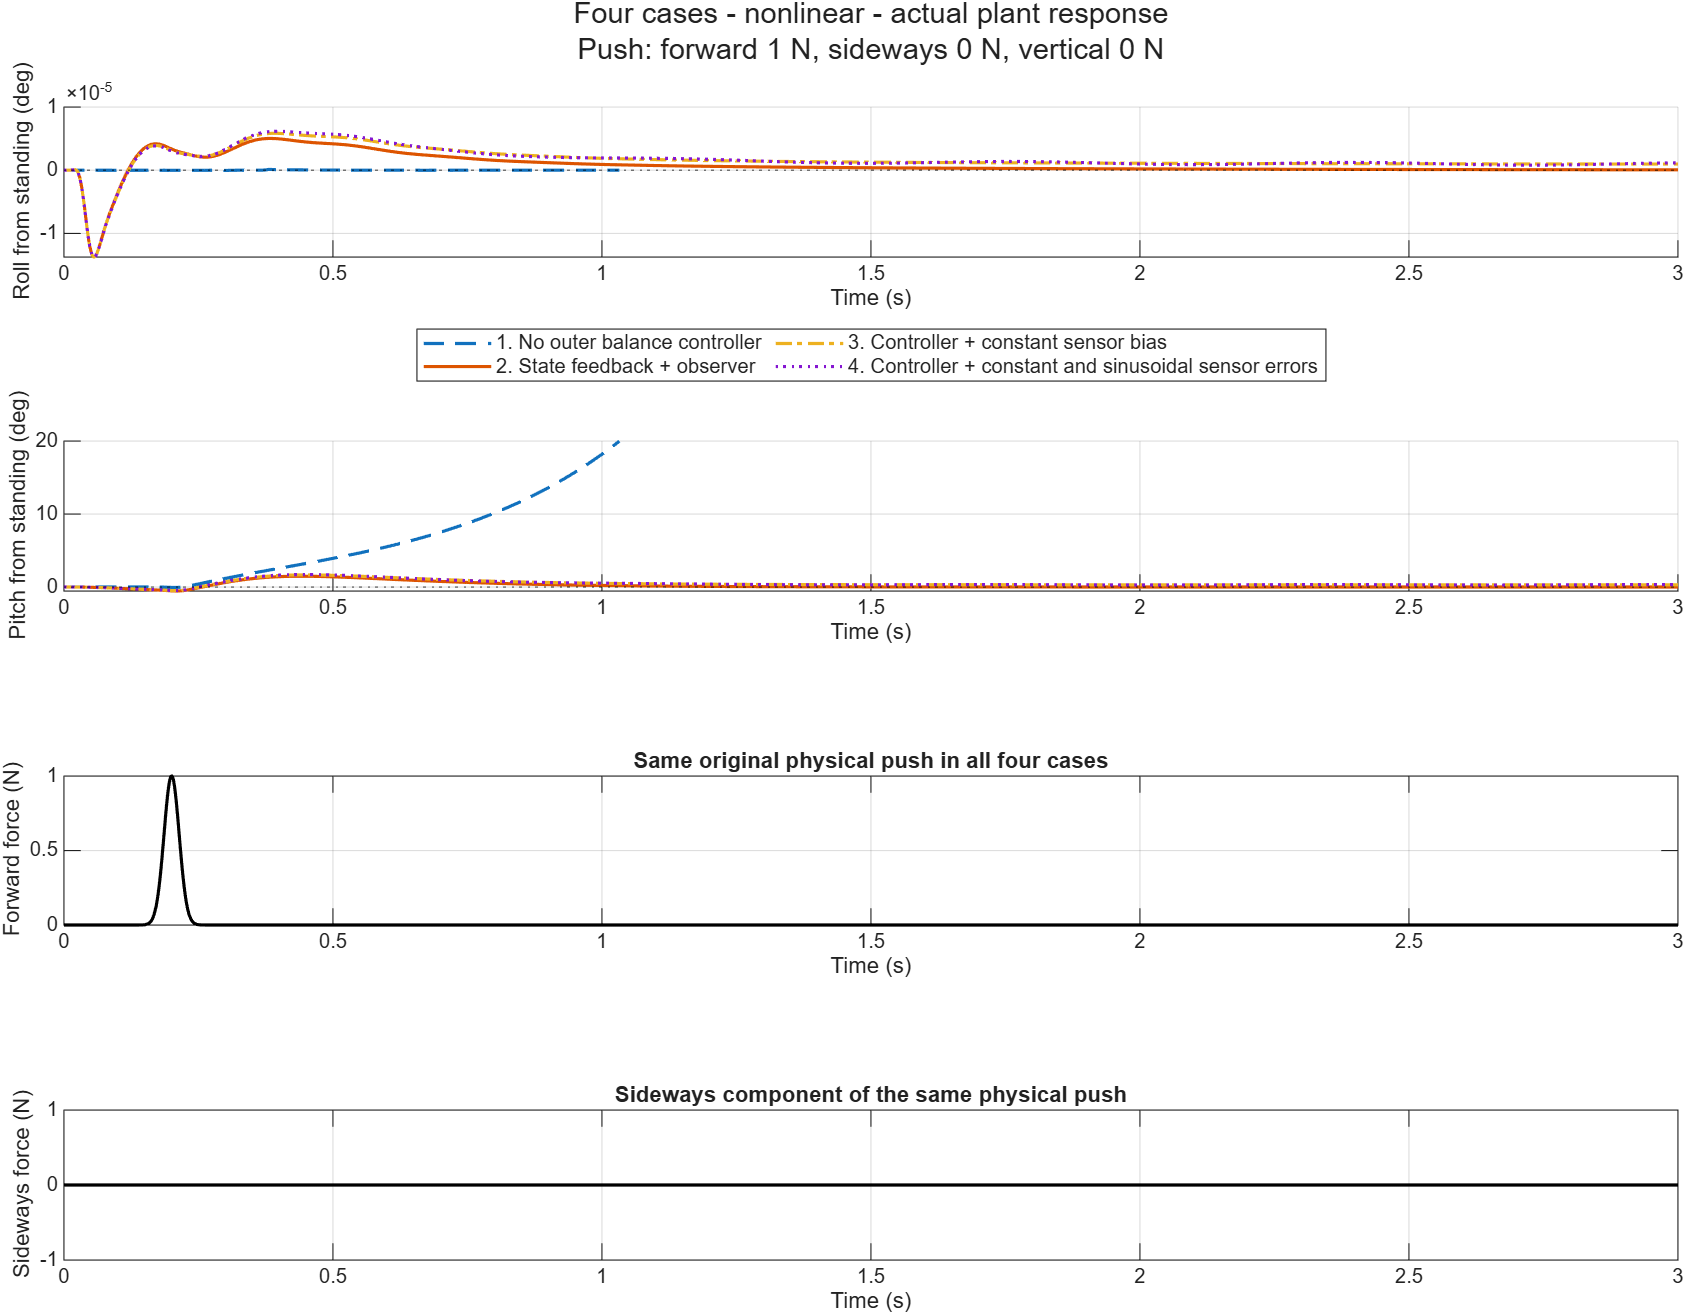
\includegraphics[width=0.485\textwidth]{figures/forward_1N_nonlinear_response.png}\hfill
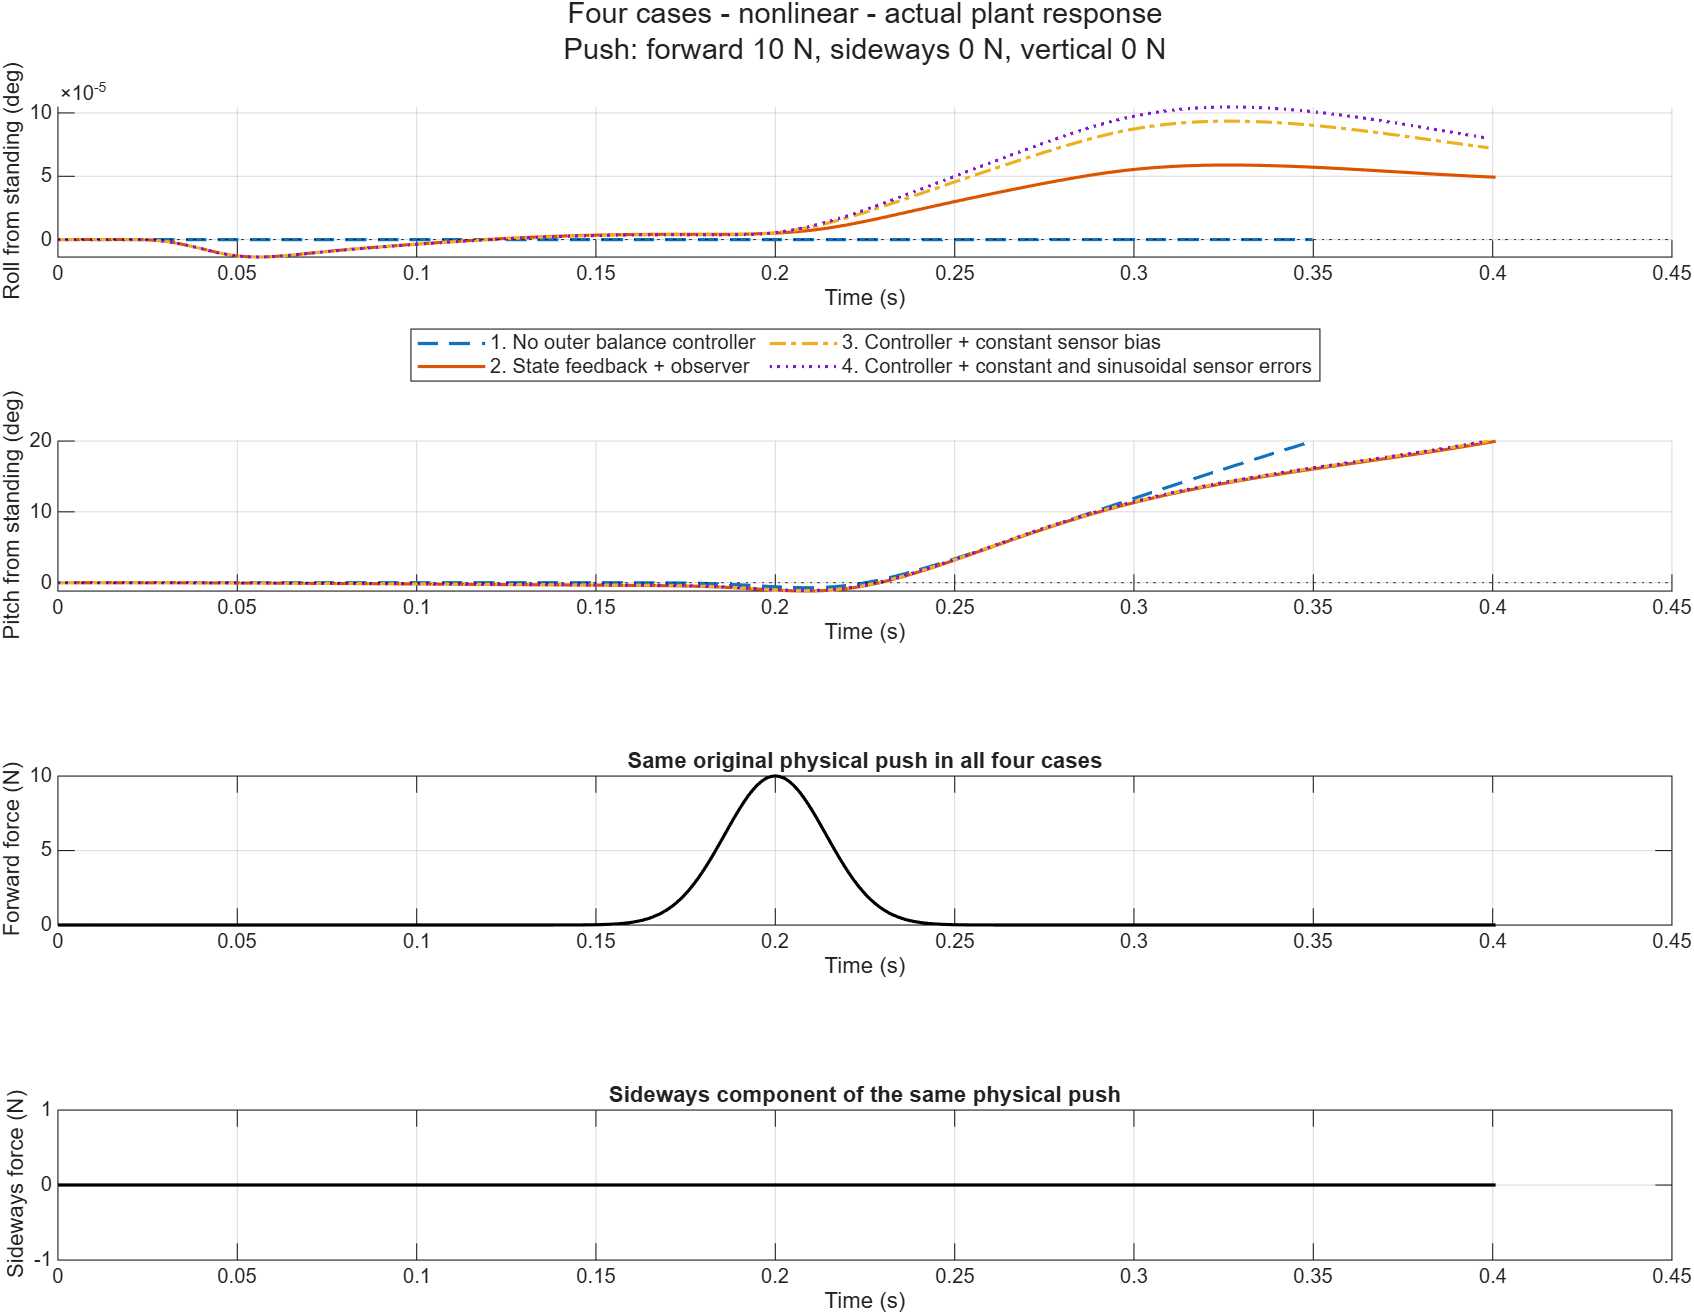
\includegraphics[width=0.485\textwidth]{figures/forward_10N_nonlinear_response.png}
\caption{Nonlinear forward-push responses at 1~N (left) and 10~N (right). All four cases receive the same force within each test. Curves ending early indicate validity termination. The 10~N run does not demonstrate recovery.}\label{fig:forward_validation}
\end{figure*}

\subsection{Sideways Recovery and Cross-Axis Behaviour}
For nonlinear B, increasing the sideways push from 1 to 5 to 10~N increases peak roll from $0.108^\circ$ to $0.855^\circ$ to $3.195^\circ$, and settling time from 0.666 to 0.824 to 1.098~s. Corresponding $t_r$ values are 0.022, 0.041 and 0.124~s, while $t_p$ values are 0.113, 0.161 and 0.314~s. Reverse-excursion ratios are 55.57\%, 51.61\% and 7.23\%. A smaller ratio at 10~N is not evidence of a smaller absolute response; both the peak and recovery time increase.

The linear B model instead predicts nearly proportional peak rolls of $0.107^\circ$, $0.537^\circ$ and $1.074^\circ$, with settling near 0.667~s for all three forces. The nonlinear 10~N roll peak is almost three times the linear prediction, showing that the local approximation understates the large-push response.

At 1~N sideways, A and B have almost identical roll peaks ($0.107^\circ$ and $0.108^\circ$). This is consistent with a naturally damped lateral response and should not be presented as a major improvement caused by outer feedback. Their pitch behaviour differs: A reaches a $3.881^\circ$ pitch excursion, compared with $0.559^\circ$ for B. At 5 and 10~N sideways, nonlinear A stops at 2.188 and 1.828~s as pitch approaches the validity limit, even though roll has largely decayed. B completes both runs; its peak pitch deviations are $0.556^\circ$ and $1.670^\circ$, respectively. Balance must therefore be judged using both axes and run completion, not the directional roll table alone.

\begin{figure*}[!t]\centering
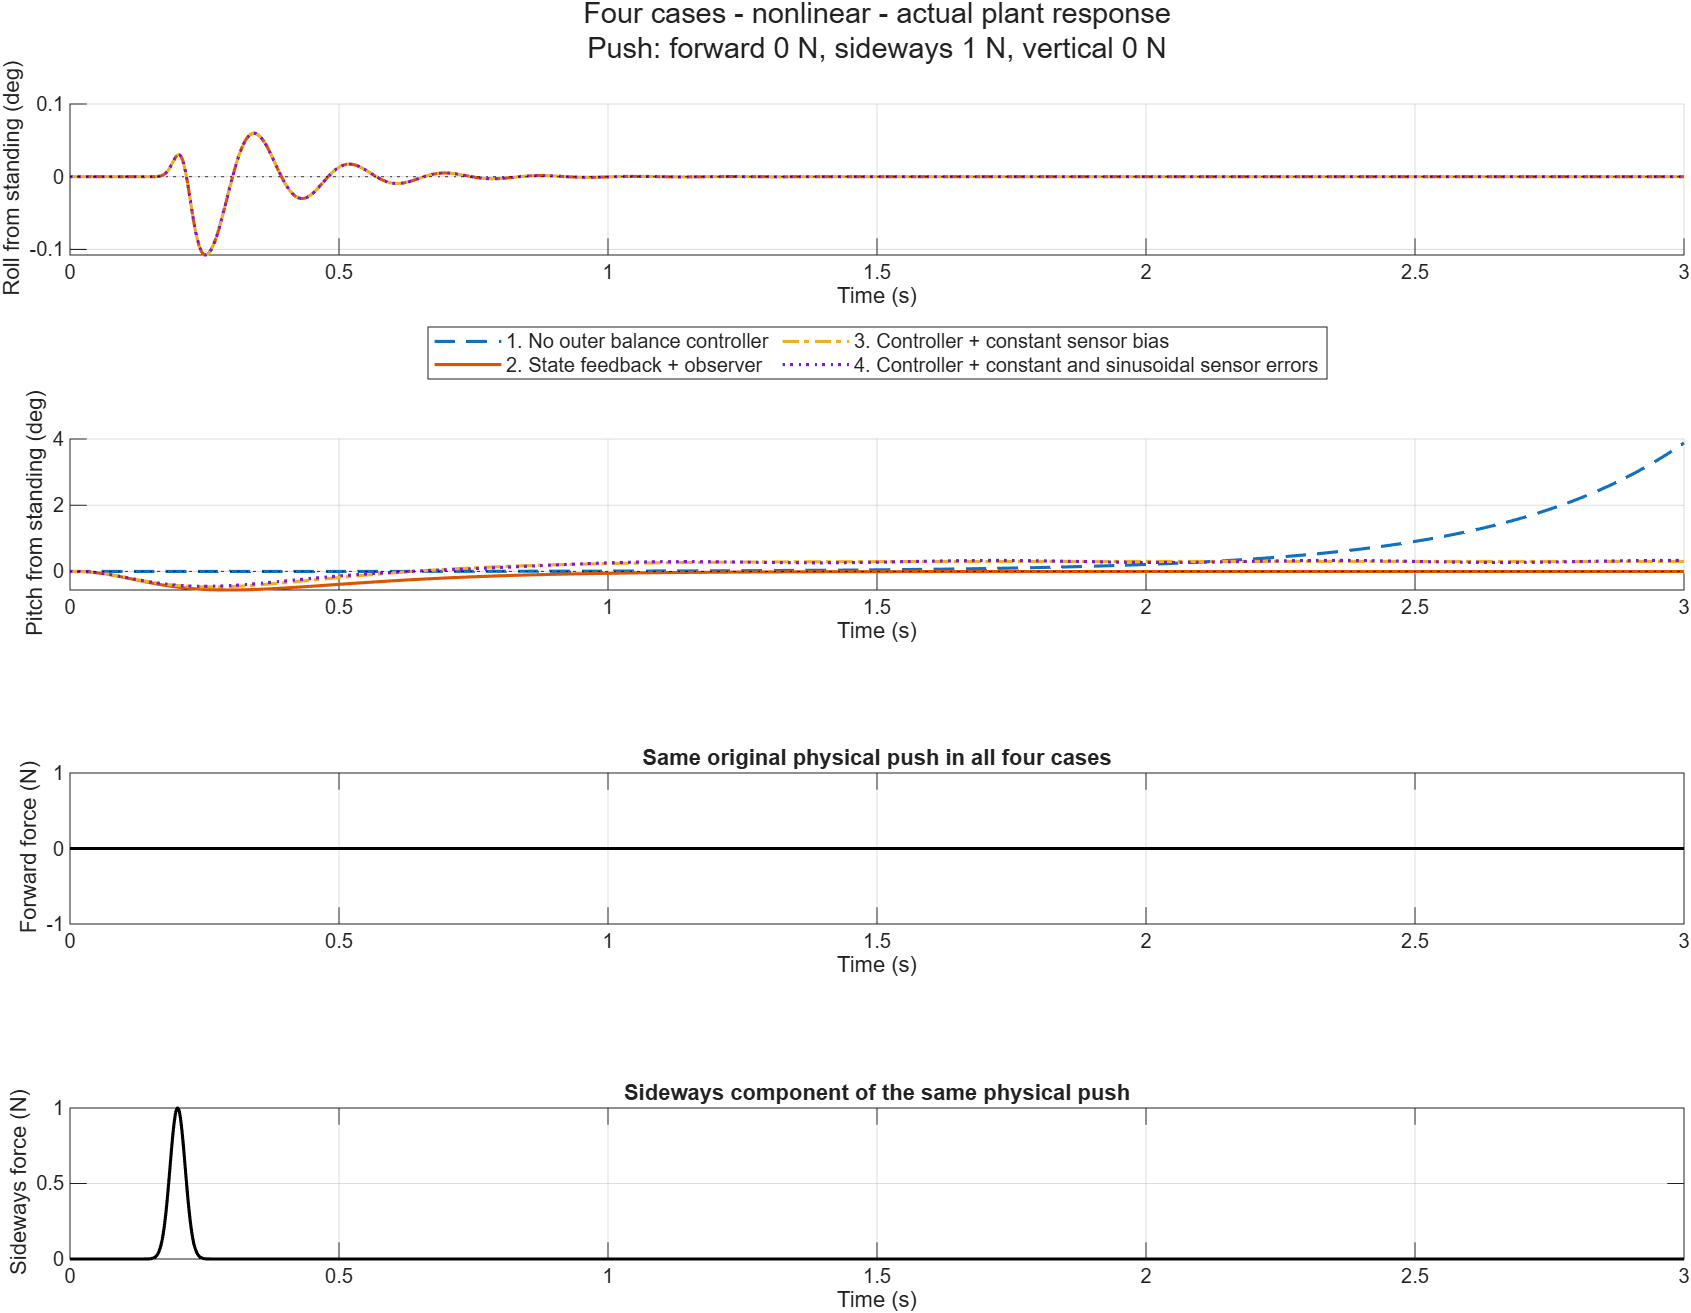
\includegraphics[width=0.485\textwidth]{figures/sideways_1N_nonlinear_response.png}\hfill
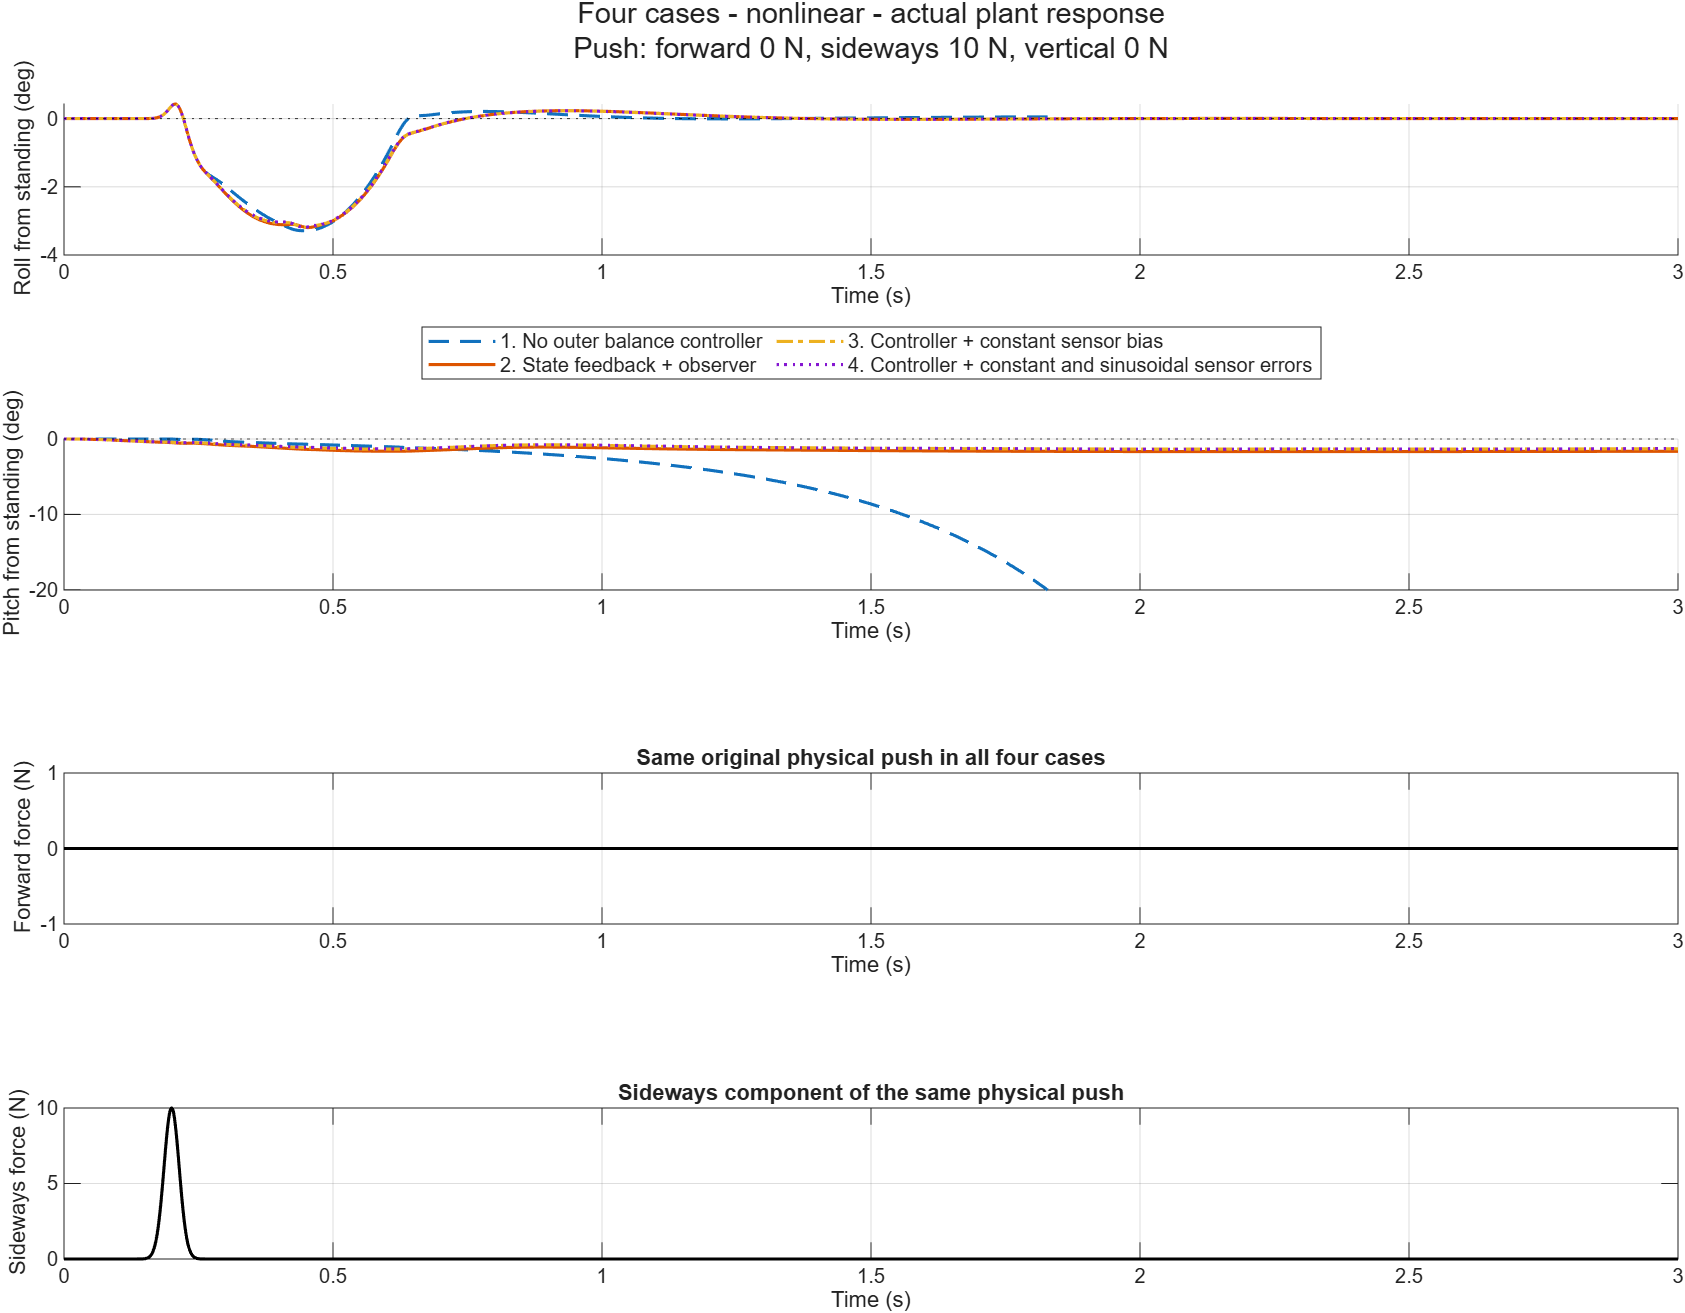
\includegraphics[width=0.485\textwidth]{figures/sideways_10N_nonlinear_response.png}
\caption{Nonlinear sideways-push responses at 1~N (left) and 10~N (right). Similar lateral traces can conceal different pitch stability. Outer feedback prevents the pitch divergence seen in the 10~N inner-servo-only case.}\label{fig:sideways_validation}
\end{figure*}

\subsection{Sensor Errors, Actuation and Scope of Validation}
For the nonlinear 1~N forward test, bias increases peak pitch from $1.474^\circ$ in B to $1.656^\circ$ in C; adding sinusoidal errors raises it to $1.708^\circ$ in D. At 3~s, C and D have pitch deviations of $0.304^\circ$ and $0.333^\circ$. Neither meets its peak-relative 2\% upright settling band. The same residual deviations appear after the 5~N forward push. Thus these sensor errors do not prevent run completion at 1 or 5~N, but they degrade upright regulation. The regulator has no integral or explicit sensor-bias estimation mechanism, so unbiased zero-error recovery cannot be inferred from nominal pole stability.

By contrast, the directional roll metrics change little between B, C and D for sideways pushes. This only establishes low sensitivity of roll to the chosen deterministic error pattern; it does not establish general IMU/encoder noise immunity. In particular, pitch offsets remain visible. Also, the linear 10~N C and D runs receive finite settling times of 1.577 and 1.647~s despite residual pitch near $0.3^\circ$: their large peaks create loose 2\% bands of approximately $0.38^\circ$. A finite peak-relative settling time is therefore not equivalent to satisfying a fixed absolute posture-error requirement.

The eight-motor plots show delivered torques, including the standing holding torque, with the $\pm0.60$~N\,m limits. The displayed nonlinear 5~N forward and 10~N sideways traces remain visibly inside those limits. The failed 10~N forward case also ends without delivered torque visibly reaching the cap. This does not prove that requested angle corrections were unclipped: the outer $\pm8^\circ$ correction limit, absolute joint-target limits and actuator lag must be assessed separately. The MAT summary contains no torque maxima, clipping durations or contact-load histories; consequently it cannot establish numerical torque margins or absence of foot lift.

\begin{figure*}[!t]\centering
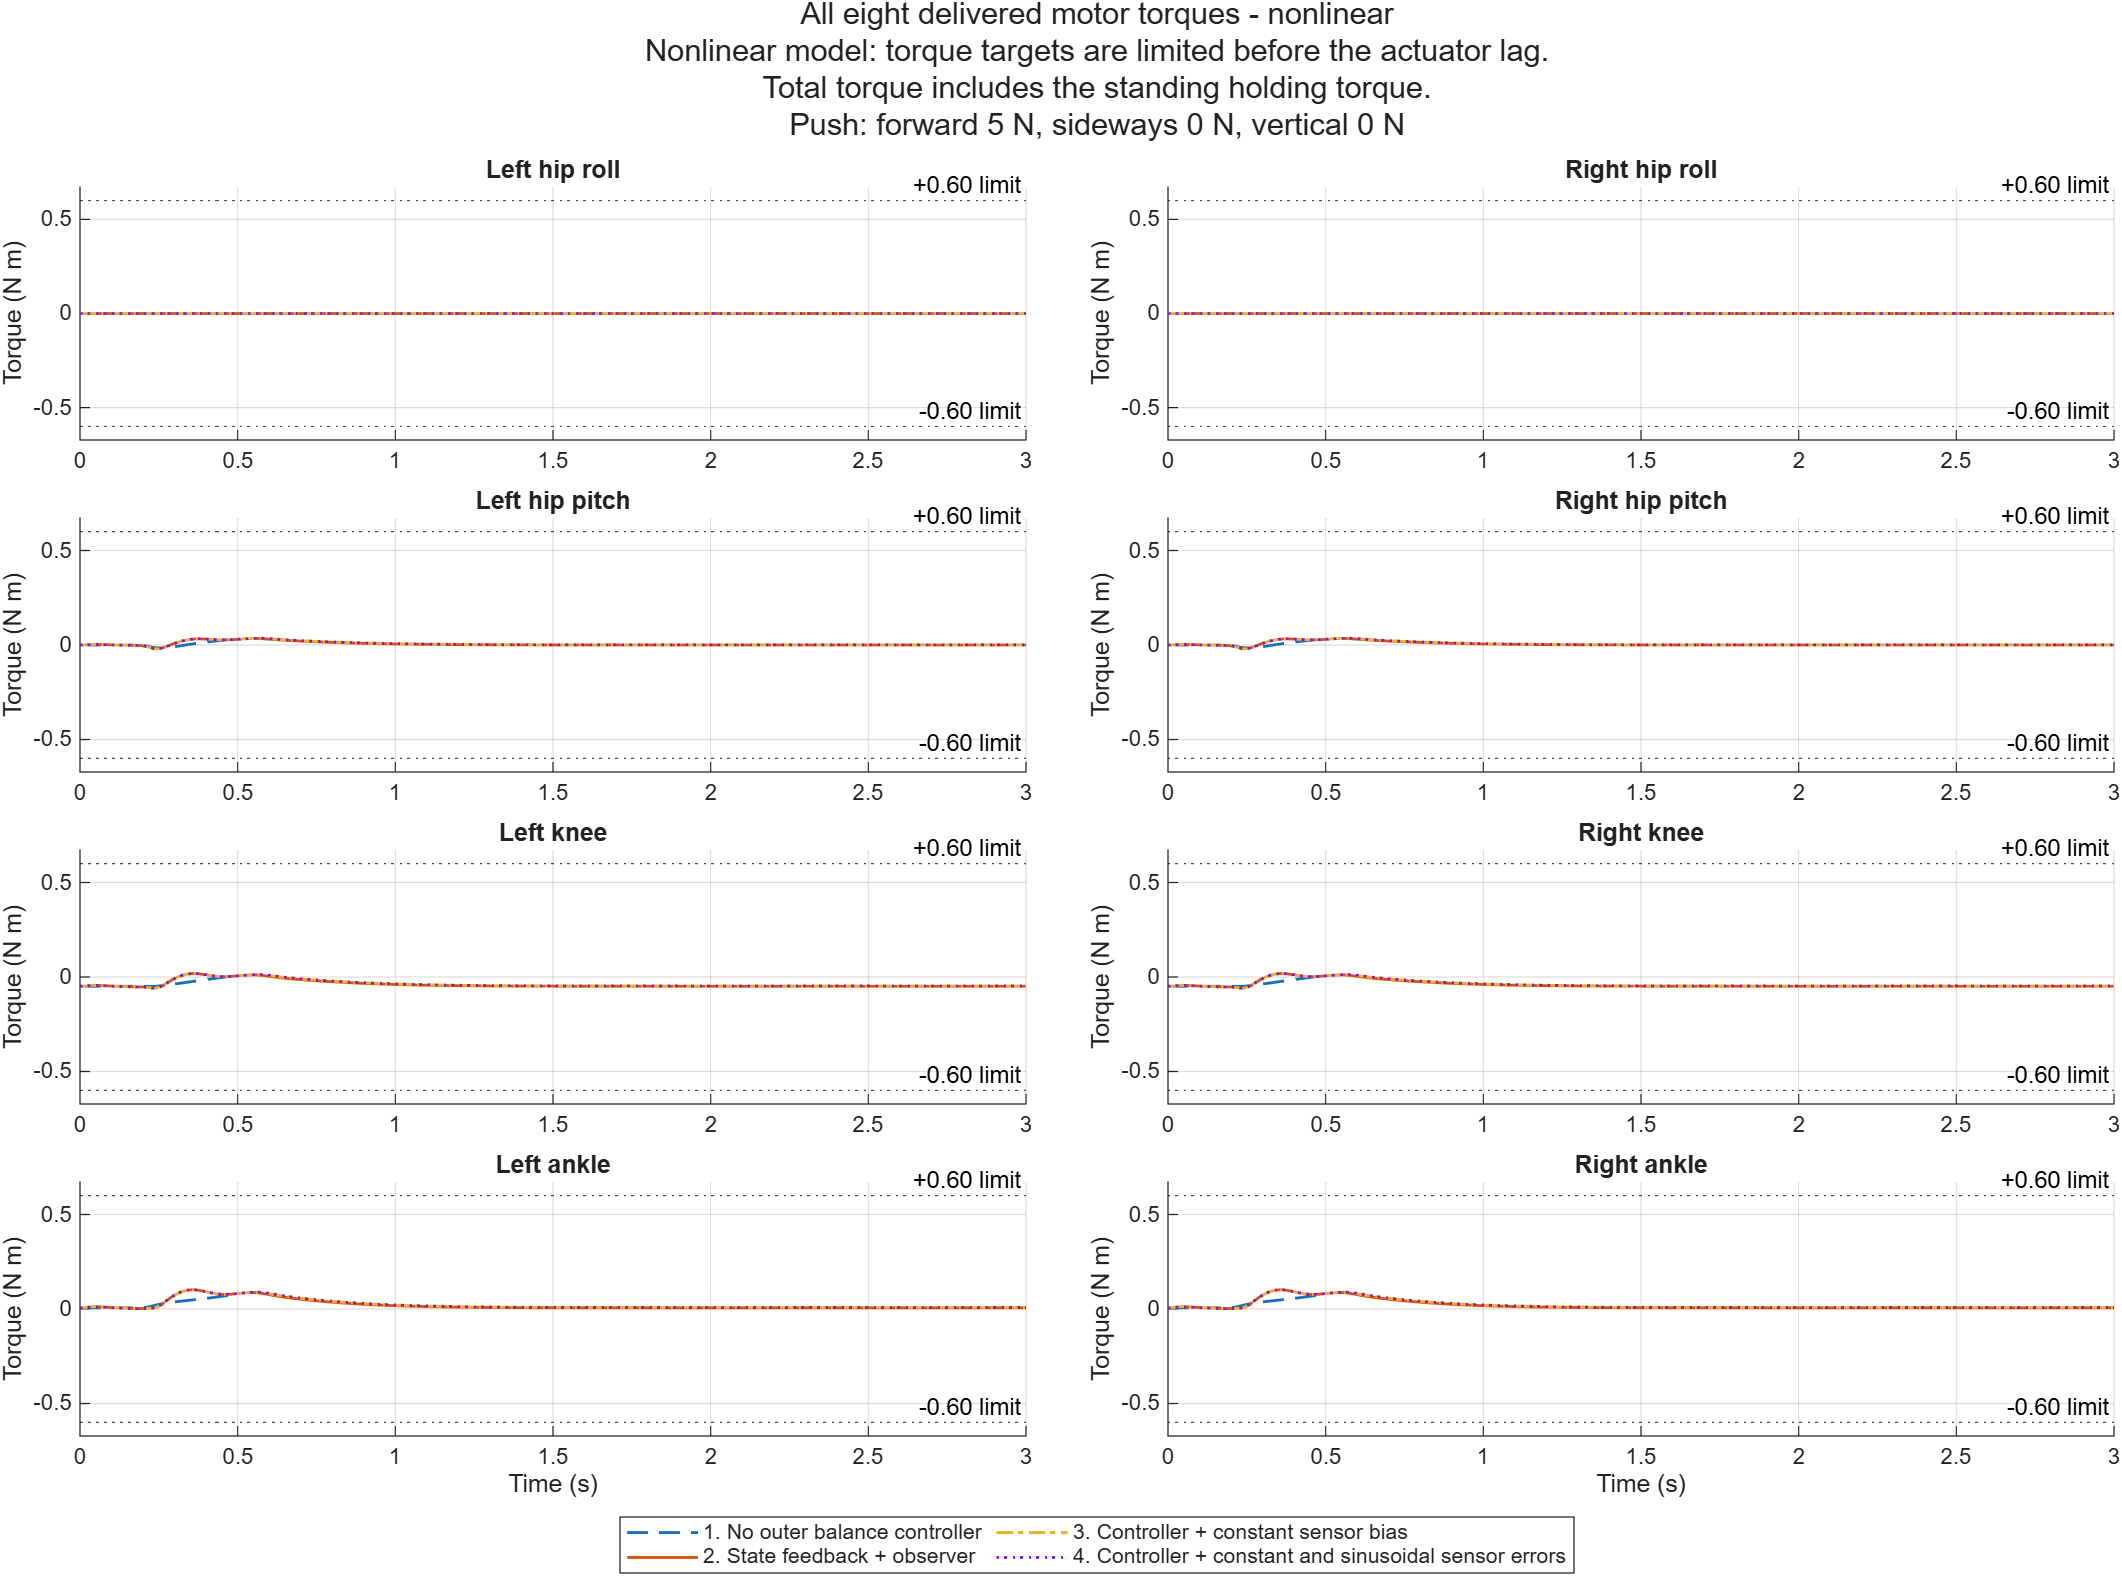
\includegraphics[width=0.485\textwidth]{figures/forward_5N_nonlinear_torques.png}\hfill
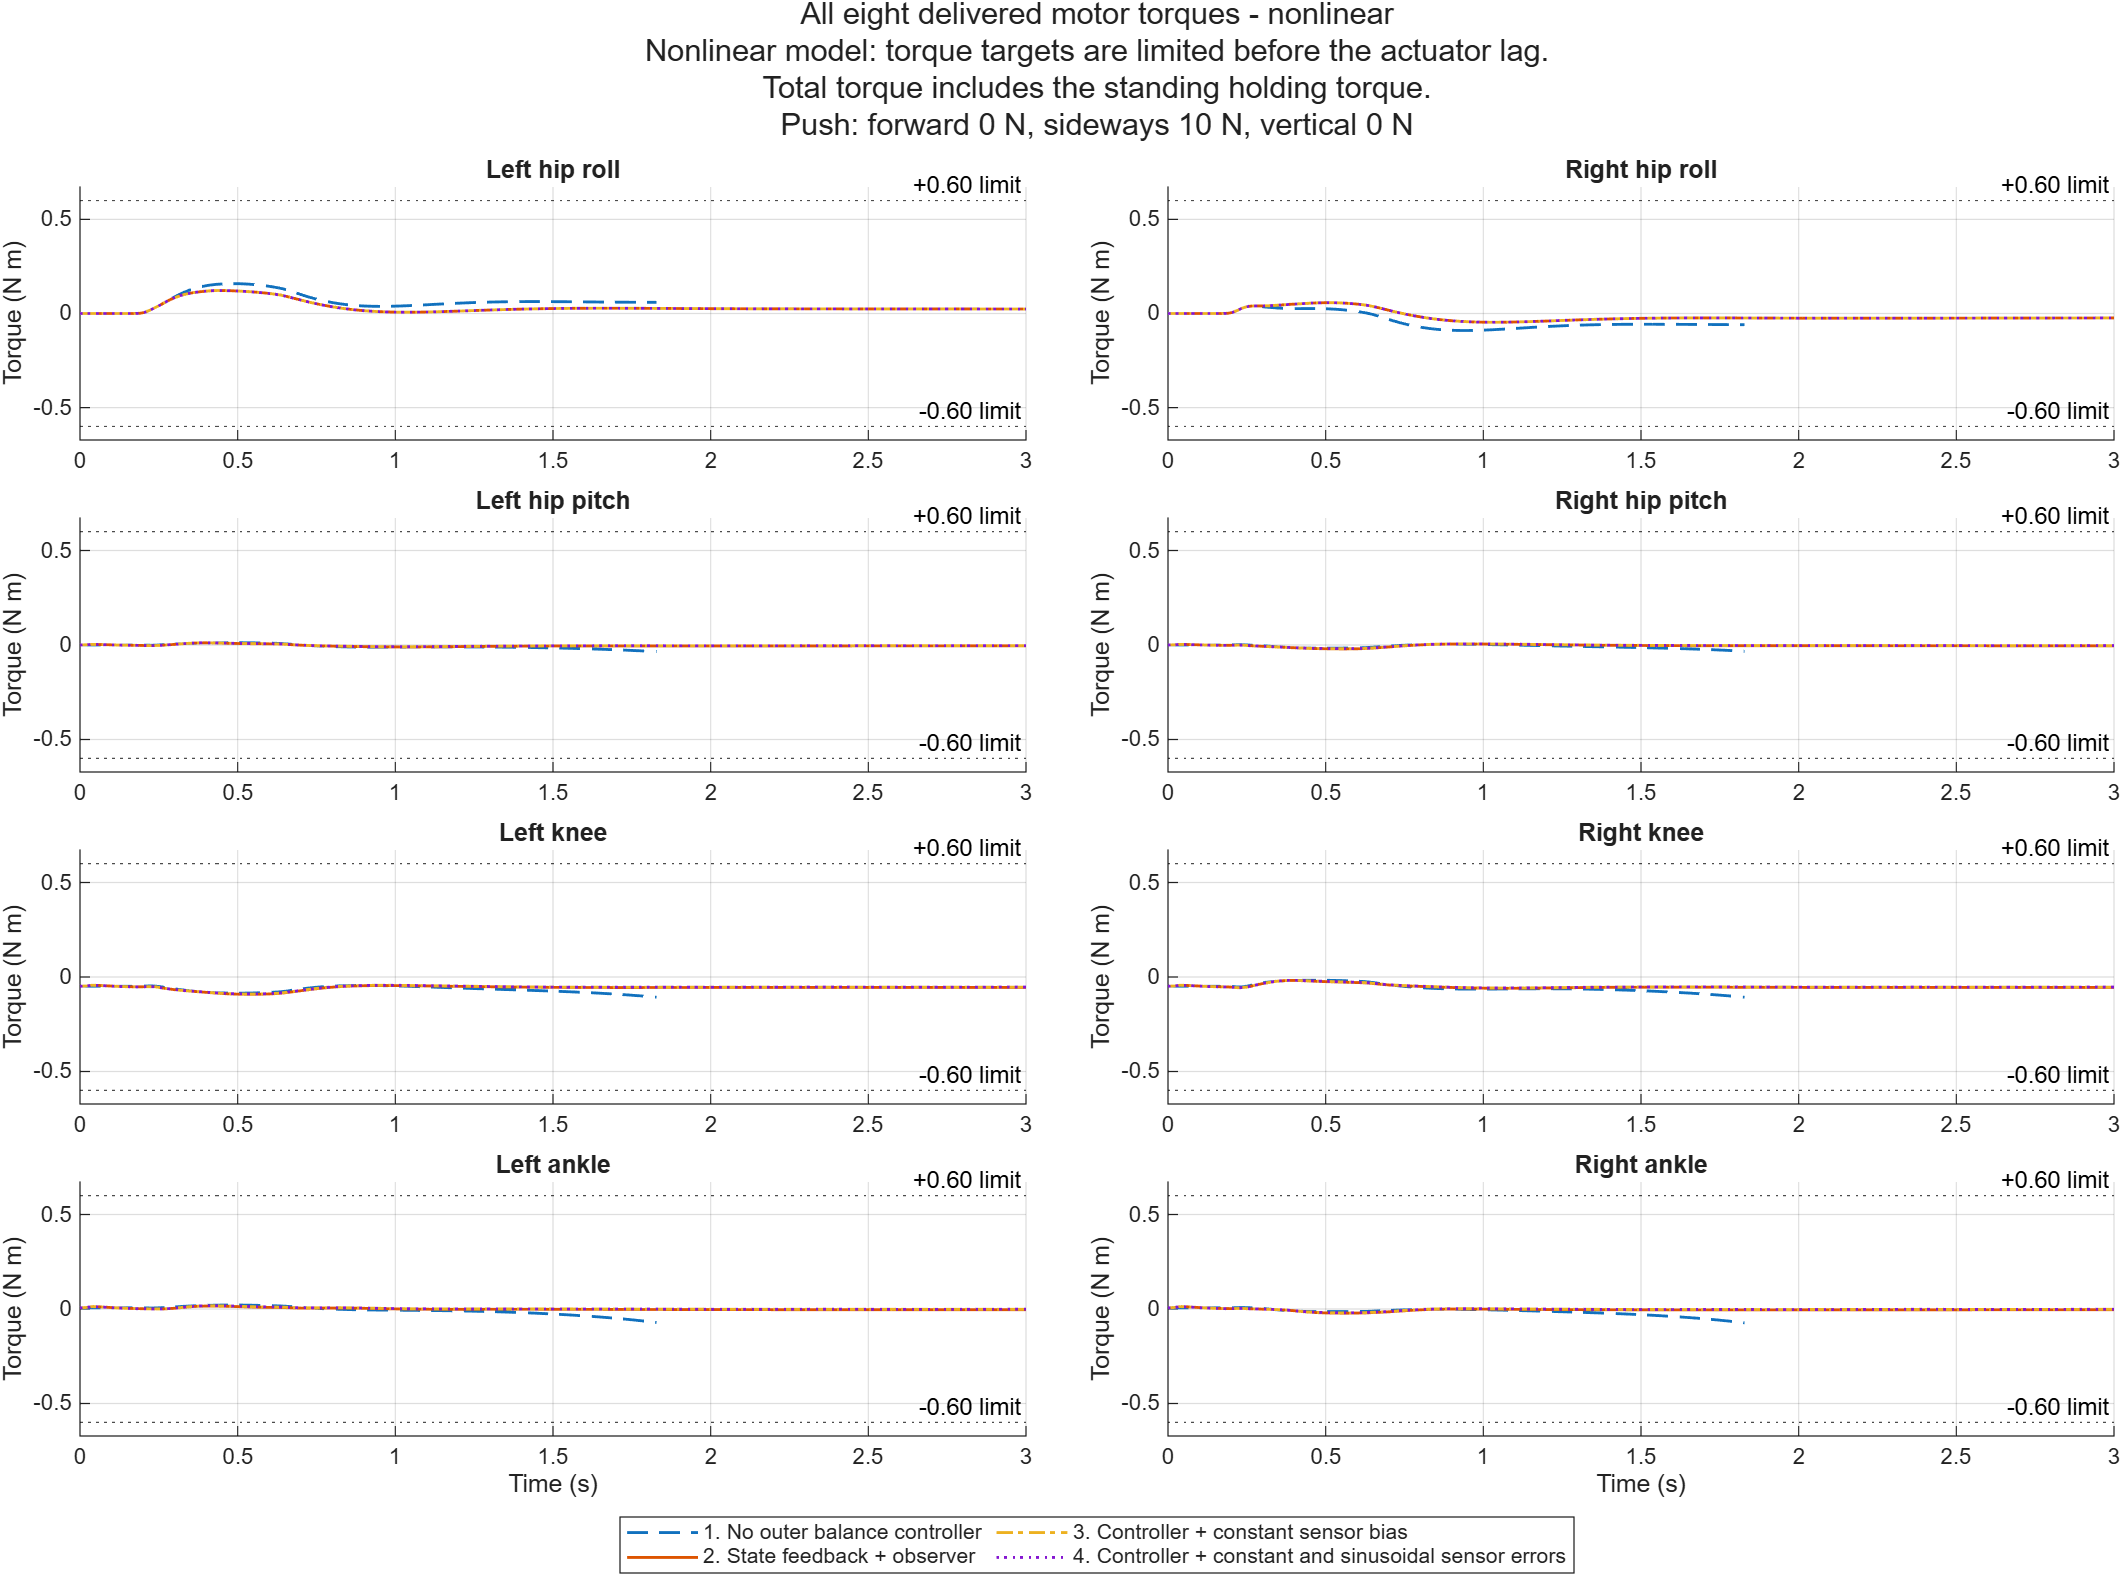
\includegraphics[width=0.485\textwidth]{figures/sideways_10N_nonlinear_torques.png}
\caption{Delivered torque for all eight motors during the nonlinear 5~N forward and 10~N sideways tests. The dotted lines indicate the motor torque caps. Torque remaining below the cap does not establish that command limits or support constraints are inactive.}\label{fig:torque_validation}
\end{figure*}

These experiments demonstrate nominal observer-based push recovery within the tested range, with clear direction-dependent limitations. The $5^\circ$ roll/pitch bound is respected in the controlled nonlinear 1~N forward and all three sideways tests, but is violated in the 5~N forward test; the 10~N forward test terminates. Settling after a push does not validate the separate $2^\circ$ initial-tilt requirement. The saved results also do not establish observer-error convergence time, uncertainty-grid robustness with fixed gains, gain/phase margins, lean-reference tracking, constant external-moment rejection, delay/backlash robustness or stochastic-noise torque statistics. These require dedicated measurements or experiments. No PID ranking, hardware-performance claim or complete satisfaction of the design criteria follows from the present batch.

\section{Conclusion}
An observer-based PID controller and a pole-placement state-feedback
controller have been formulated for standing balance of an articulated
MicroDuck model. Both generate coordinated targets for eight leg servos at
50~Hz and reconstruct a 33-state balance vector from one six-axis IMU and
eight joint-angle channels. The remaining three global-pose coordinates are
outside the regulation objective. The design therefore connects body-level
balance to individual servo action while preserving actuator lag and contact
physics in nonlinear evaluation.

The two approaches offer different capabilities. PID provides an explicit
integral mechanism for feasible constant-disturbance rejection and a
configurable posture reference, but depends on a chosen joint allocation and
requires saturation management. Pole placement gives direct control of the
selected nominal balance modes while preserving fast stable modes; the
supplied regulator does not by itself provide integral disturbance rejection
or lean tracking. In both cases, observer initialisation, sampling and model
mismatch affect the transient response and must be included in the comparison.

\textbf{Final result statement to complete:} Across [insert number] common
nonlinear tests, [insert controller] achieved [insert settling time], [insert
peak tilt] and [insert torque/contact margin]. Criteria [insert IDs] were met;
criteria [insert IDs] were not met or remain untested. This conclusion must
be based on matched plant parameters and limits, rather than the different
default demonstrations.

The current scope is simulated standing and push recovery, not walking,
stepping or demonstrated hardware balance. Remaining limitations include
assumed actuator parameters, a local observer model, simplified contact and
unverified sensor-error distributions. The next steps are to freeze a
hardware-supported plant configuration, complete the common validation
matrix, calibrate actuator and sensor parameters and then test constrained
operation on hardware. No hardware robustness or complete satisfaction of
C1--C10 is claimed from source code alone.

\appendix
\subsection{Sensor and Servo-Error Settings}\label{app:sensors}
Gyroscope readings are quantised at $0.0175^\circ$/s per LSB and clipped at $\pm500^\circ$/s as optional readout approximations~\cite{openmicroduck_params}. The datasheet profile uses the densities in the System Model section over an assumed 25~Hz bandwidth; the stress profile uses $2^\circ$/s and 0.1~m/s$^2$. Servo-side errors can also be enabled: command jitter $0.05^\circ$, feedback position error $0.02^\circ$, feedback velocity error $0.1^\circ$/s and torque noise 1~mN\,m. Unlike sensor noise, these change the body motion. Sensor noise, servo errors and calibration uncertainty are configured independently and are disabled in the nominal configuration.



\section*{Acknowledgment}
Claude and ChatGPT were used during the preparation of this report to assist with clarifying and refining written content, drafting and developing MATLAB code, and conducting final checks for accuracy, consistency and correctness. AI-generated suggestions and outputs were reviewed by the authors and used where appropriate in the preparation of this report.


\bibliographystyle{IEEEtran}
\bibliography{references}

\end{document}
